\documentclass[10pt, oneside]{article} % The default font size and one-sided printing (no margin offsets)

\usepackage[spanish]{babel}
\usepackage{subfig}
\usepackage{titlesec}
\usepackage{array}
\usepackage{graphicx}
\usepackage{float}
\newcolumntype{L}[1]{>{\raggedright\let\newline\\\arraybackslash\hspace{0pt}}m{#1}}
\newcolumntype{C}[1]{>{\centering\let\newline\\\arraybackslash\hspace{0pt}}m{#1}}
\newcolumntype{R}[1]{>{\raggedleft\let\newline\\\arraybackslash\hspace{0pt}}m{#1}}

\begin{document}
 
\section{CuZr a distintas temperaturas}

\subsection{Compresion}

\begin{figure}[H]
\centering
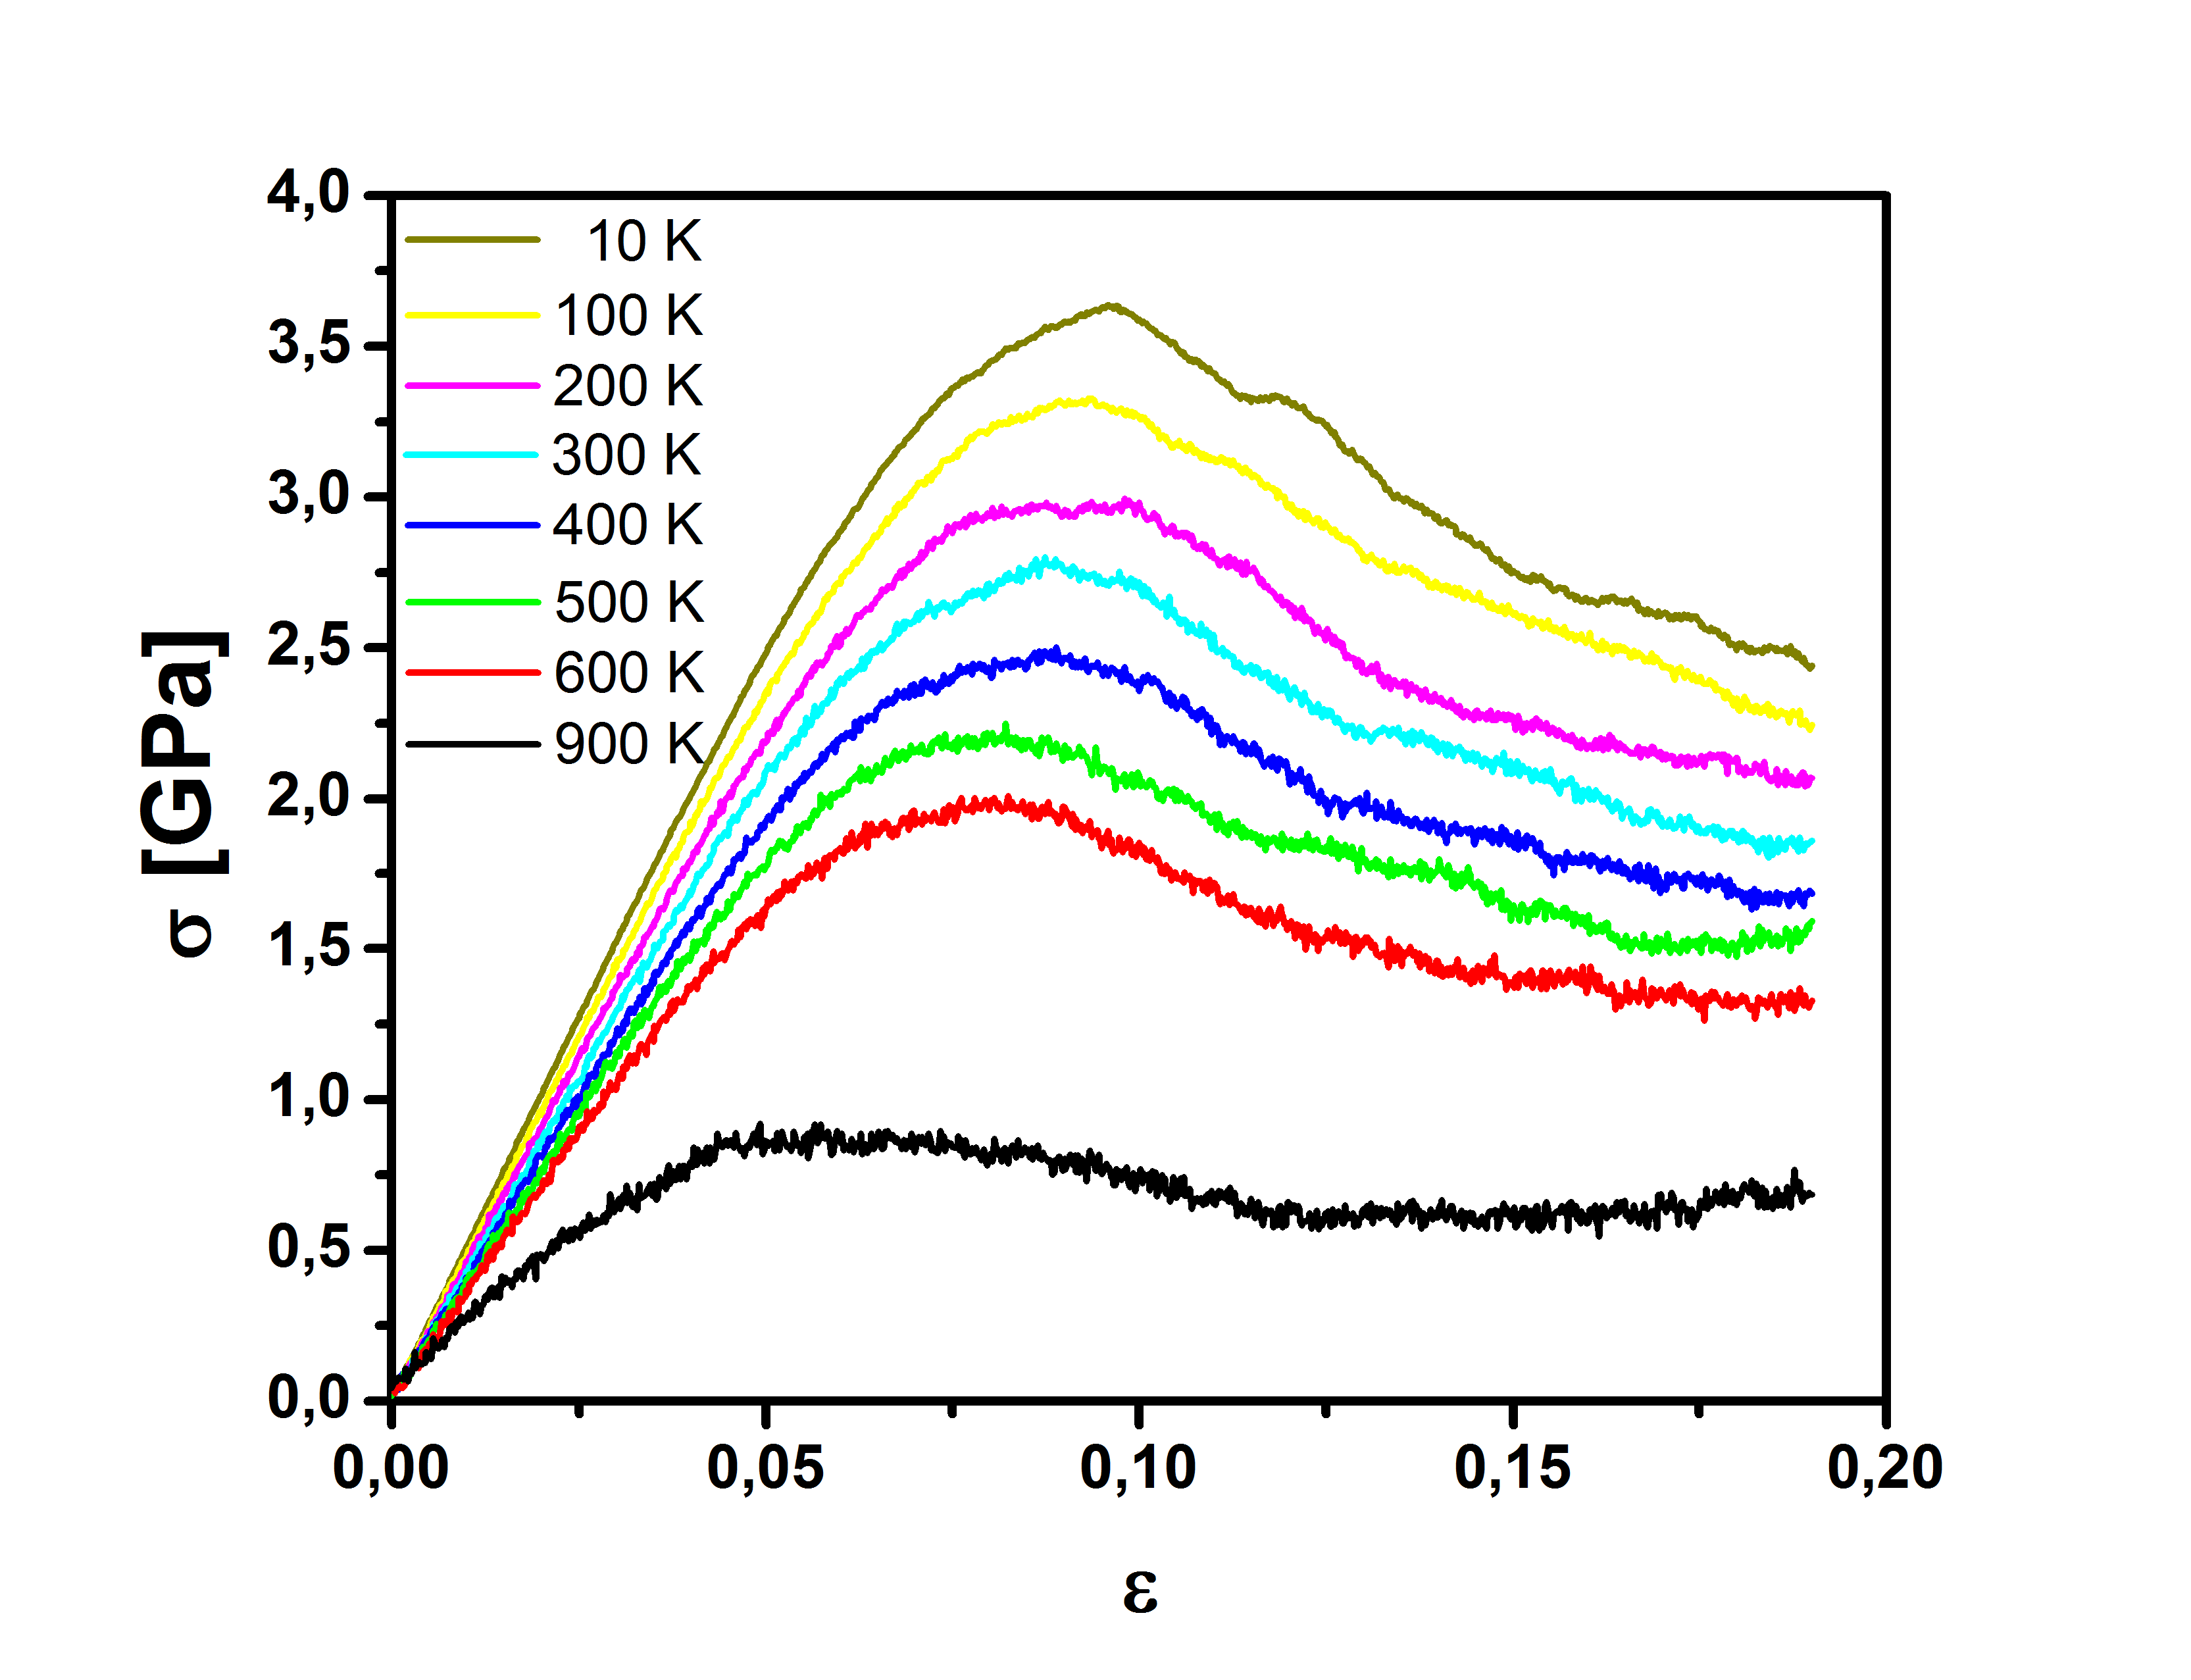
\includegraphics[width=8cm]{stress_strain_COMP.png}
\caption{Von Mises vs. strain}
\end{figure}

\begin{figure}[H]
\centering
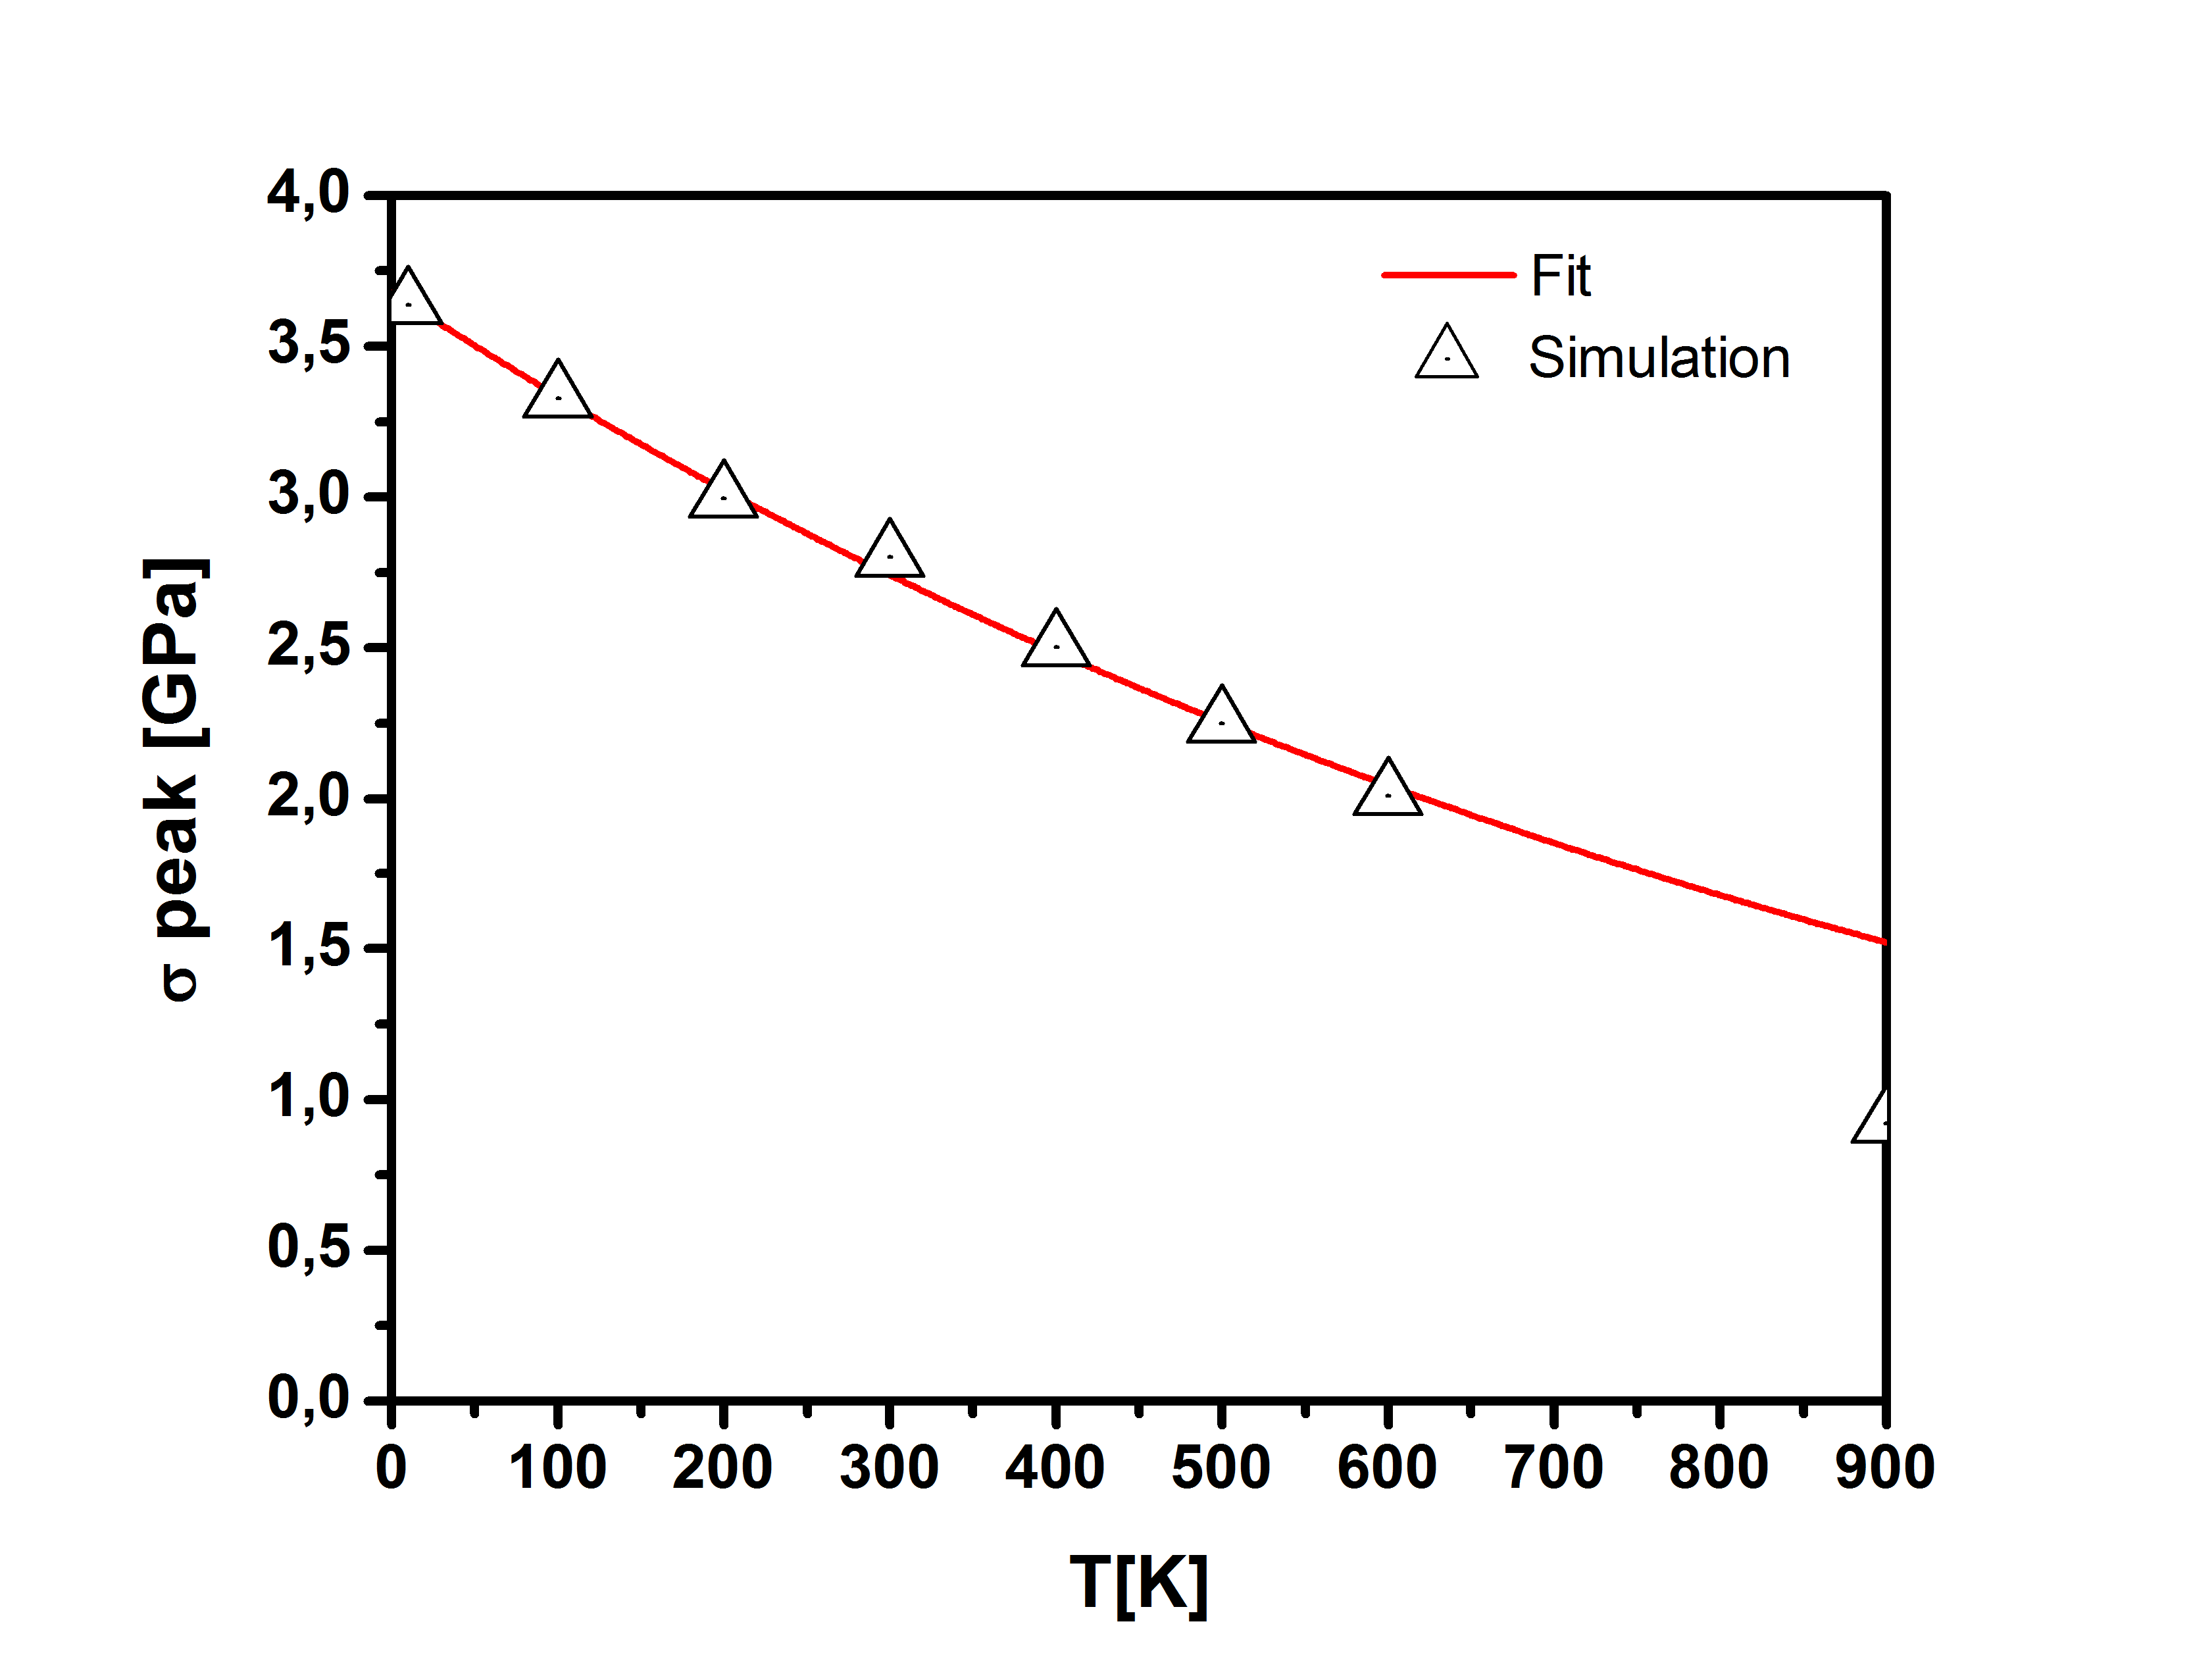
\includegraphics[width=8cm]{peakstress_T_COMP.png}
\caption{Von Mises maximo vs. Temperatura}
\end{figure}

\begin{figure}[H]
\centering
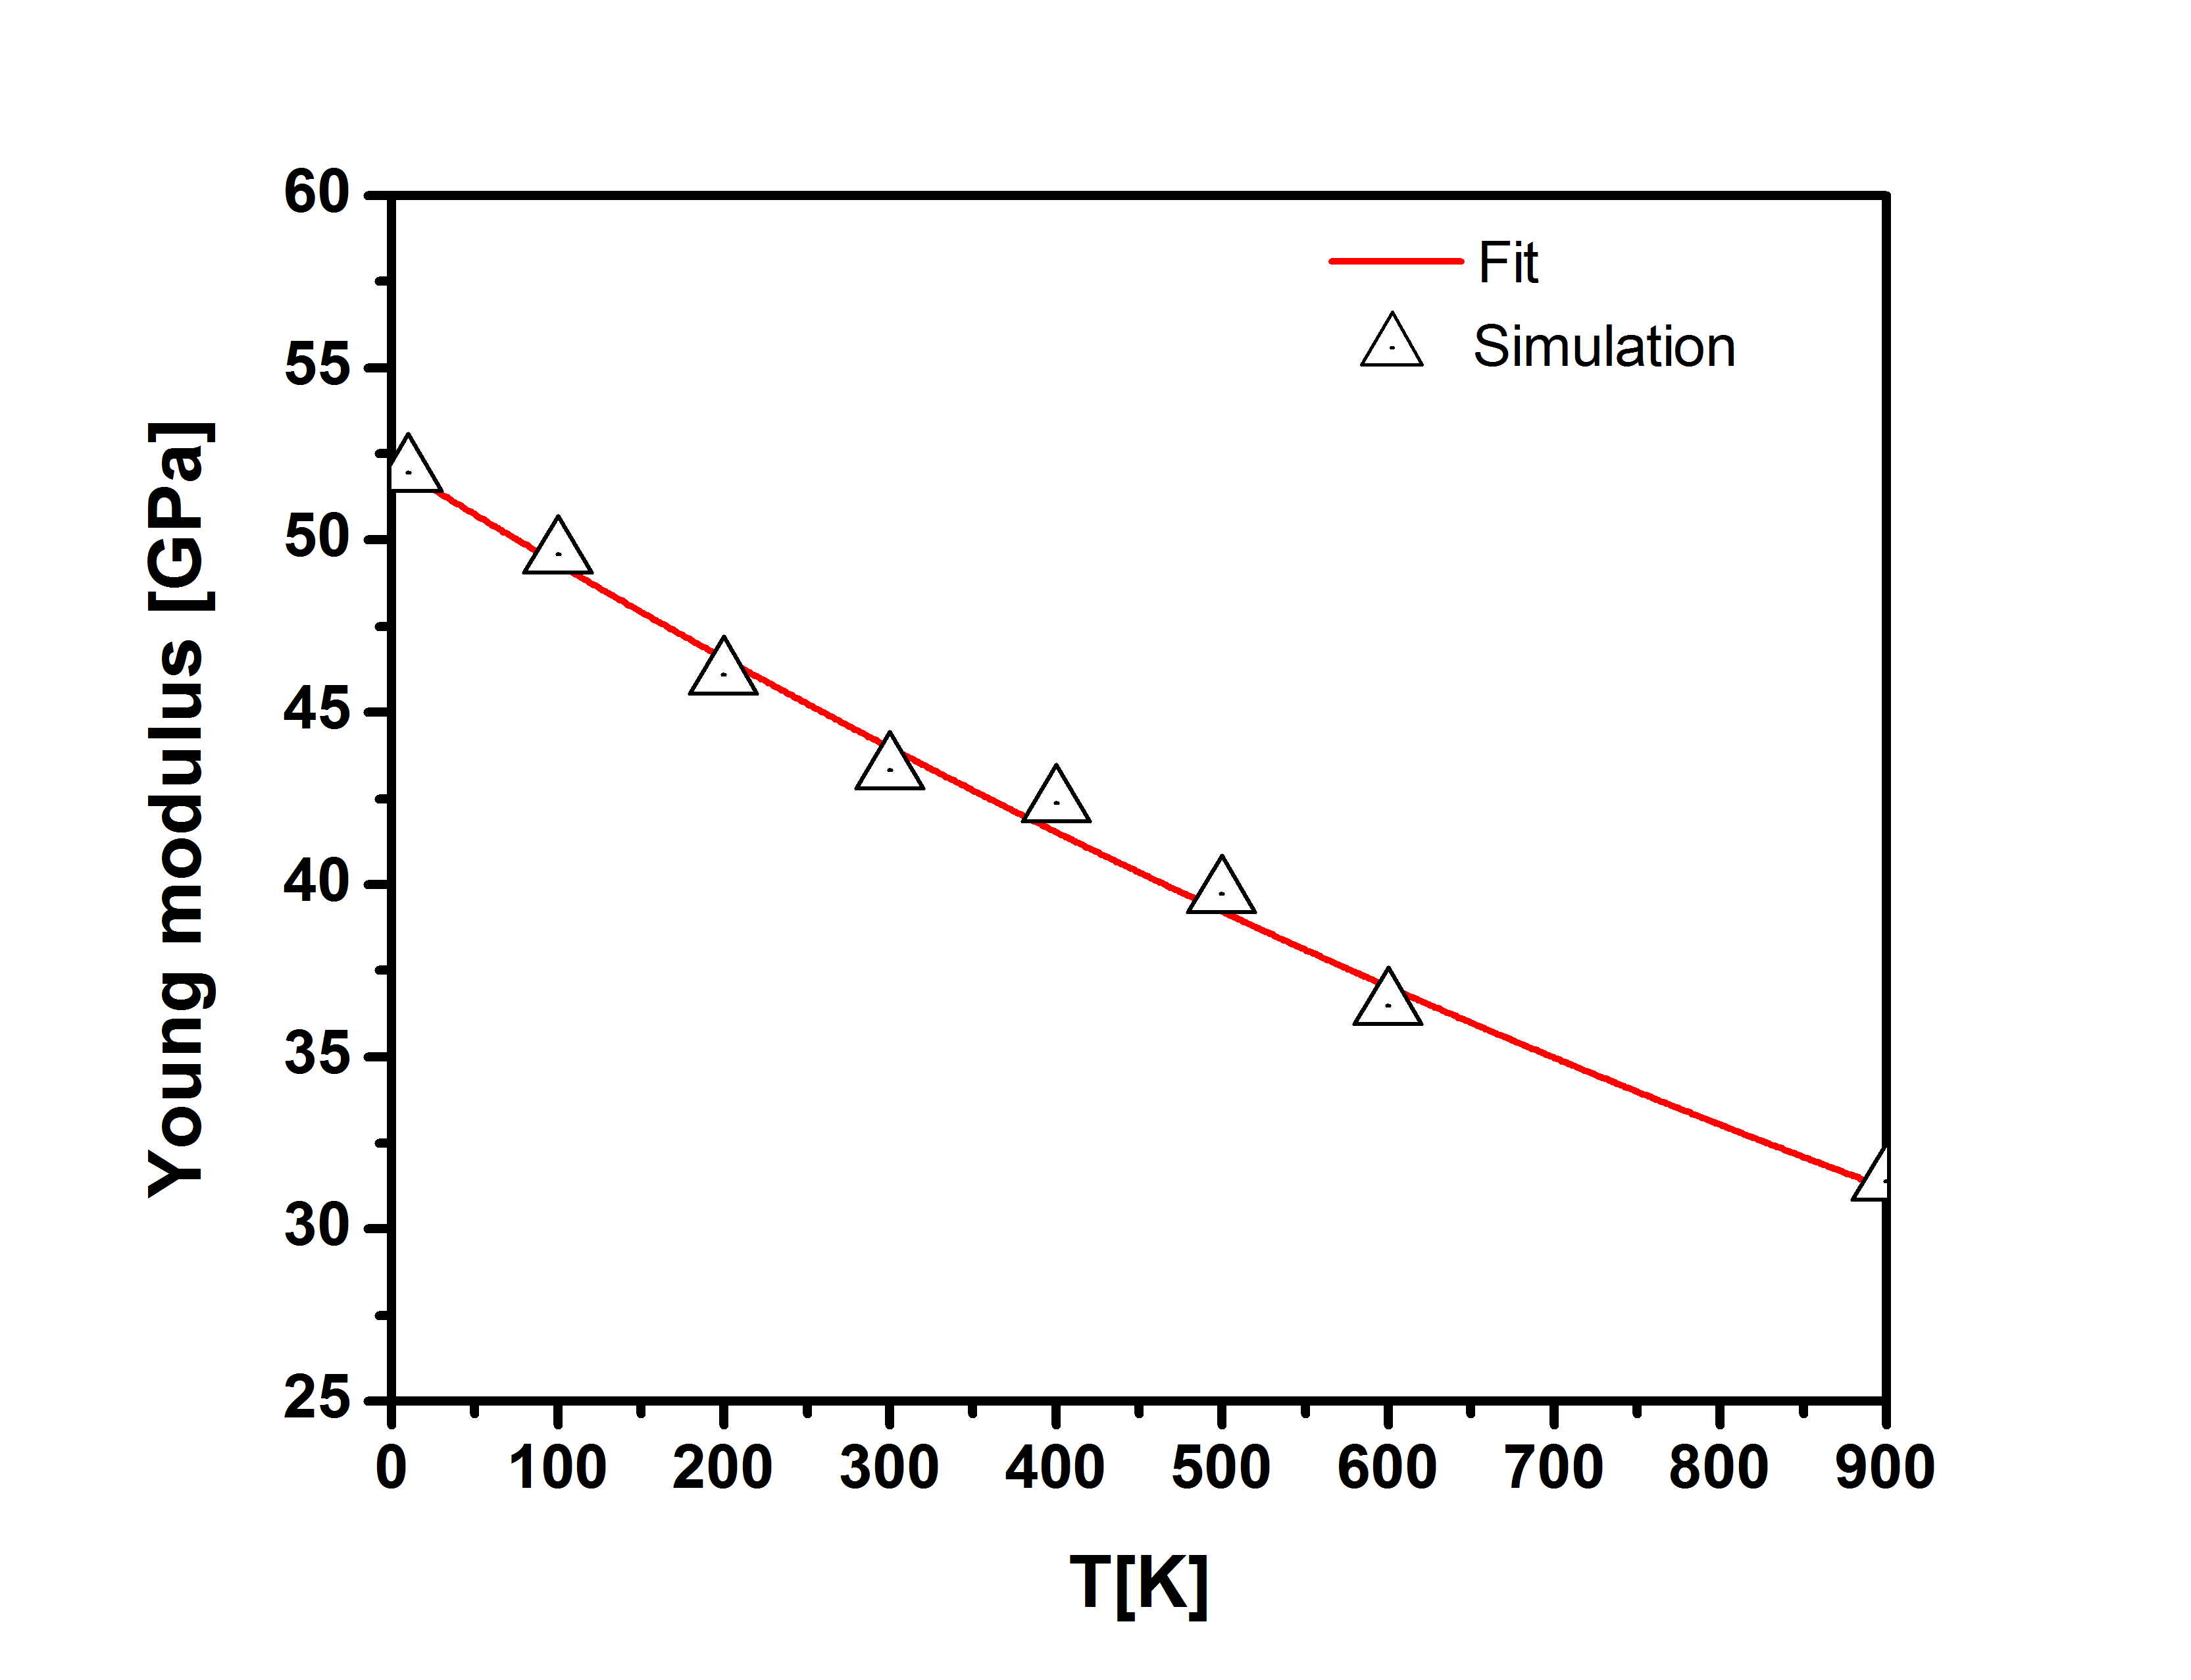
\includegraphics[width=8cm]{young_T_COMP.png}
\caption{Modulo Young vs. Temperatura}
\end{figure}

\subsection{Traccion}

\begin{figure}[H]
\centering
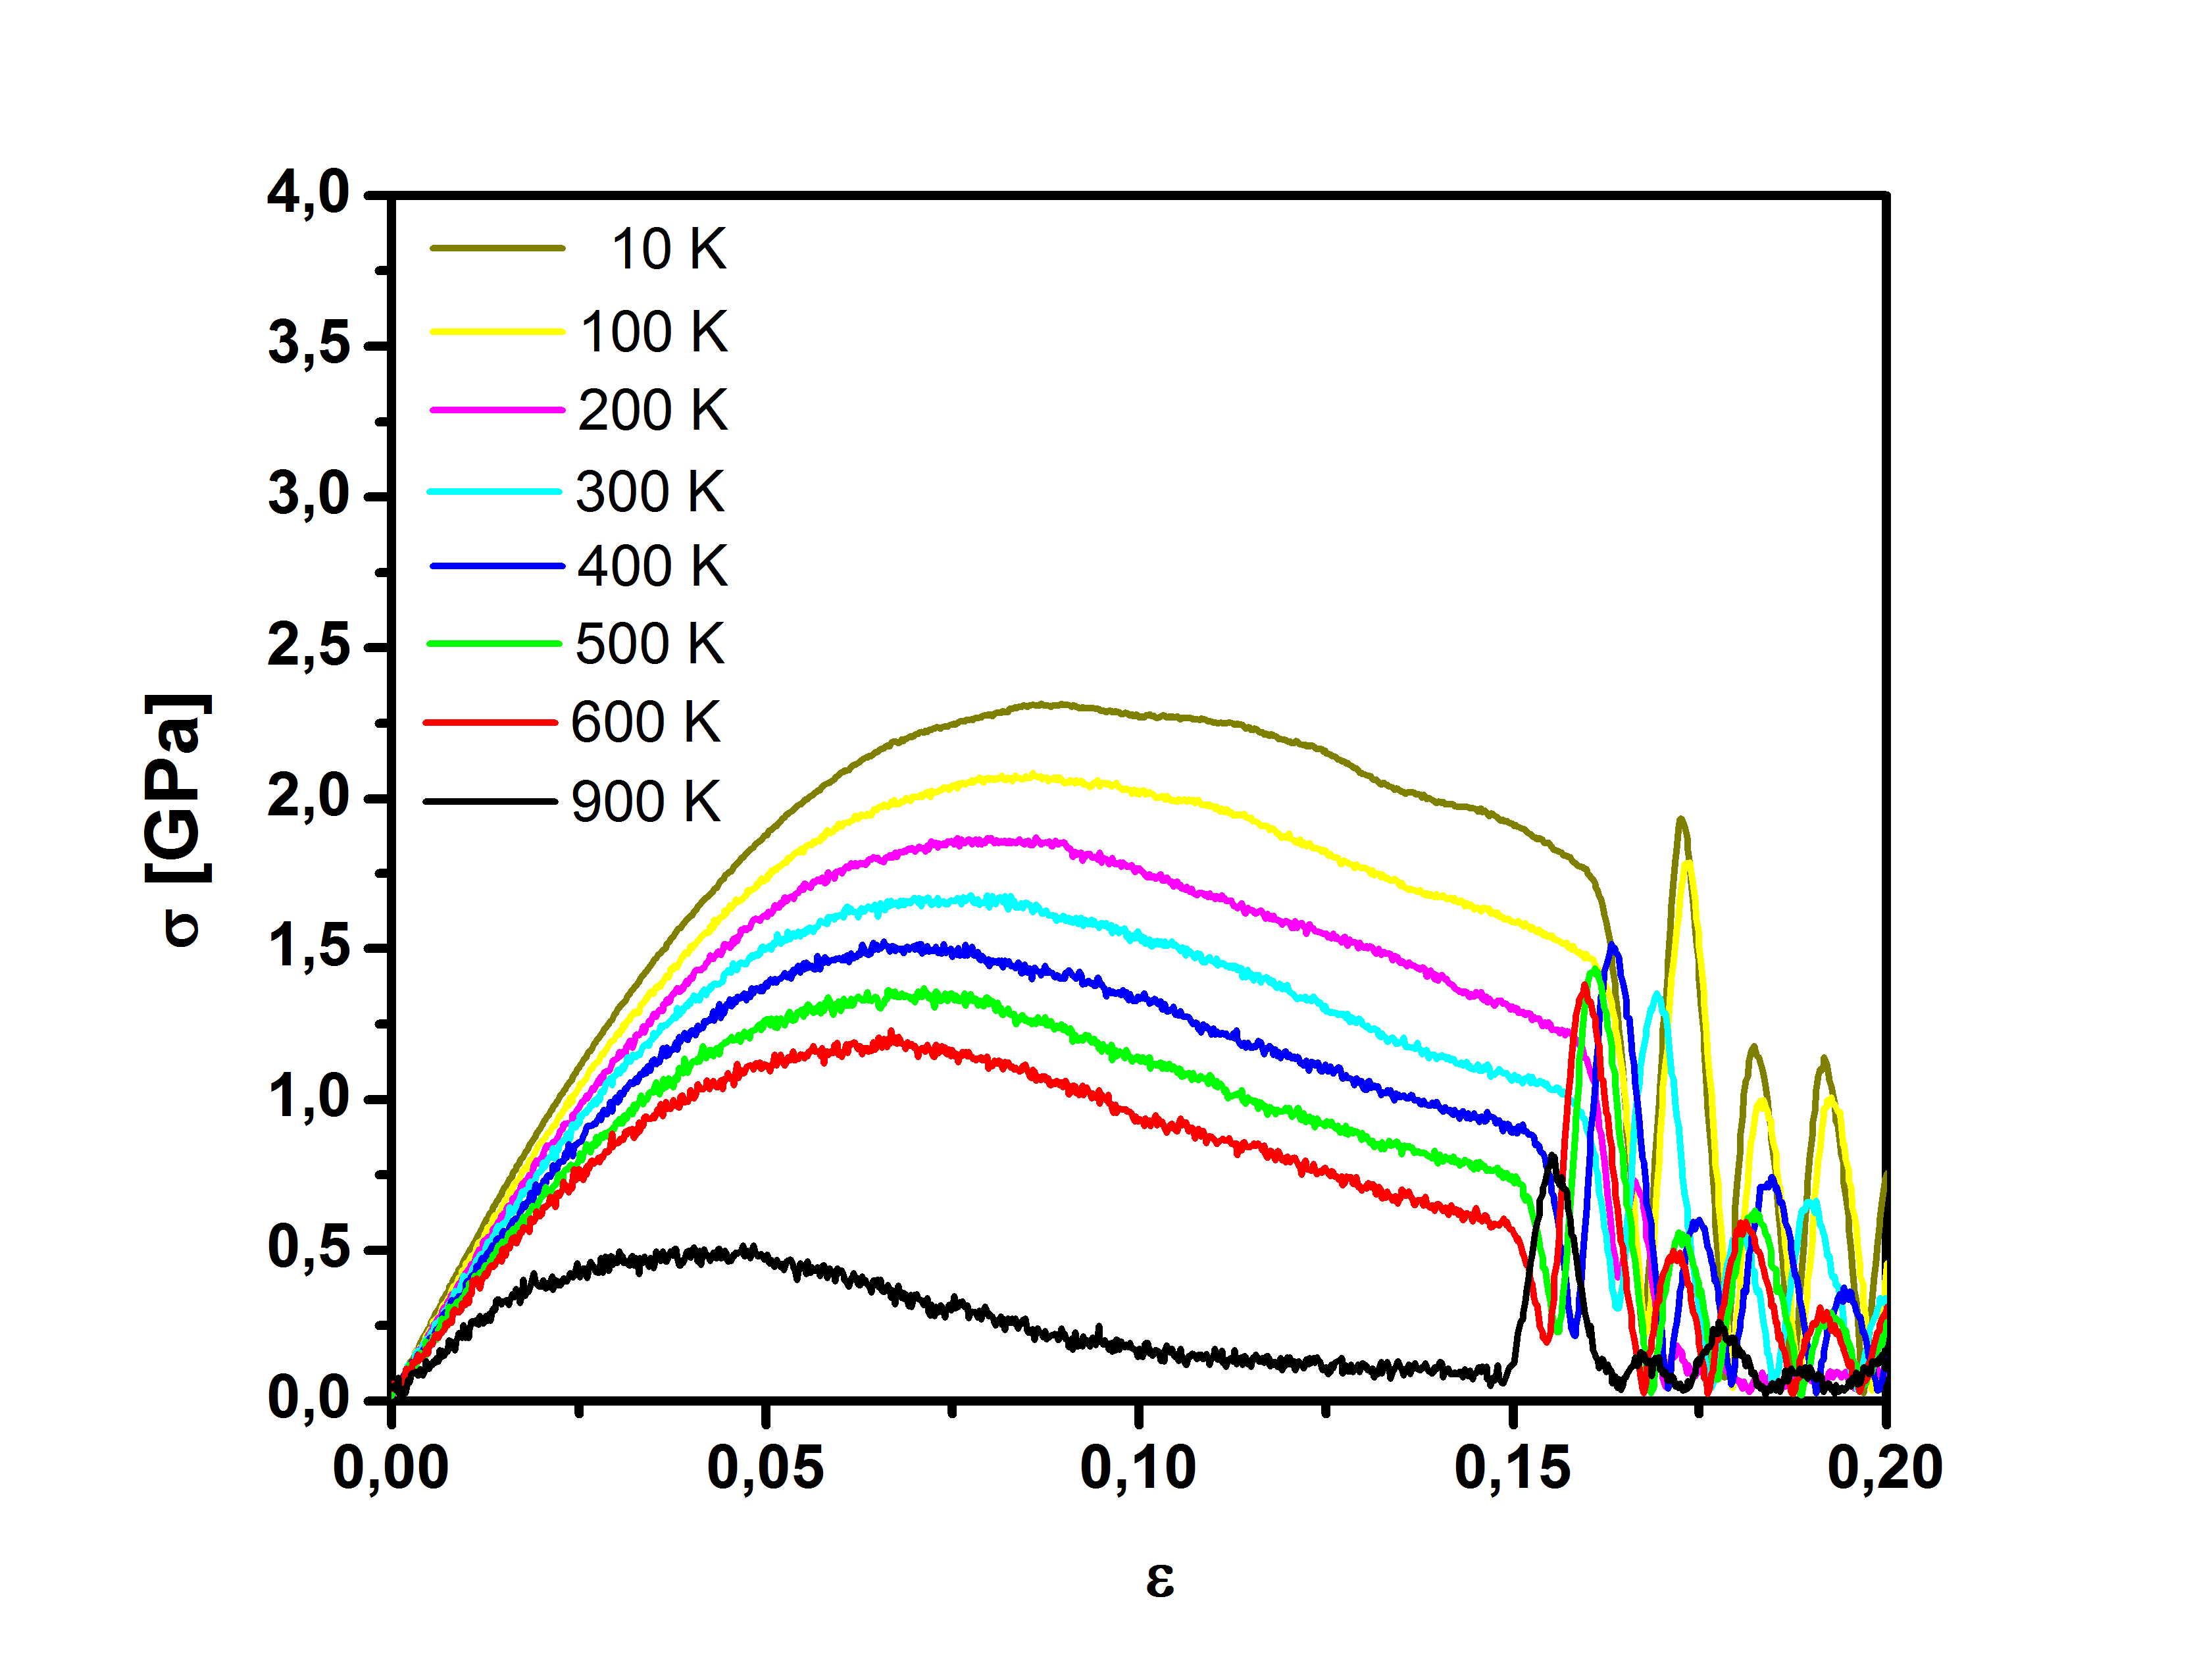
\includegraphics[width=8cm]{stress_strain_TEN.png}
\caption{Von Mises vs. strain}
\end{figure}

\begin{figure}[H]
\centering
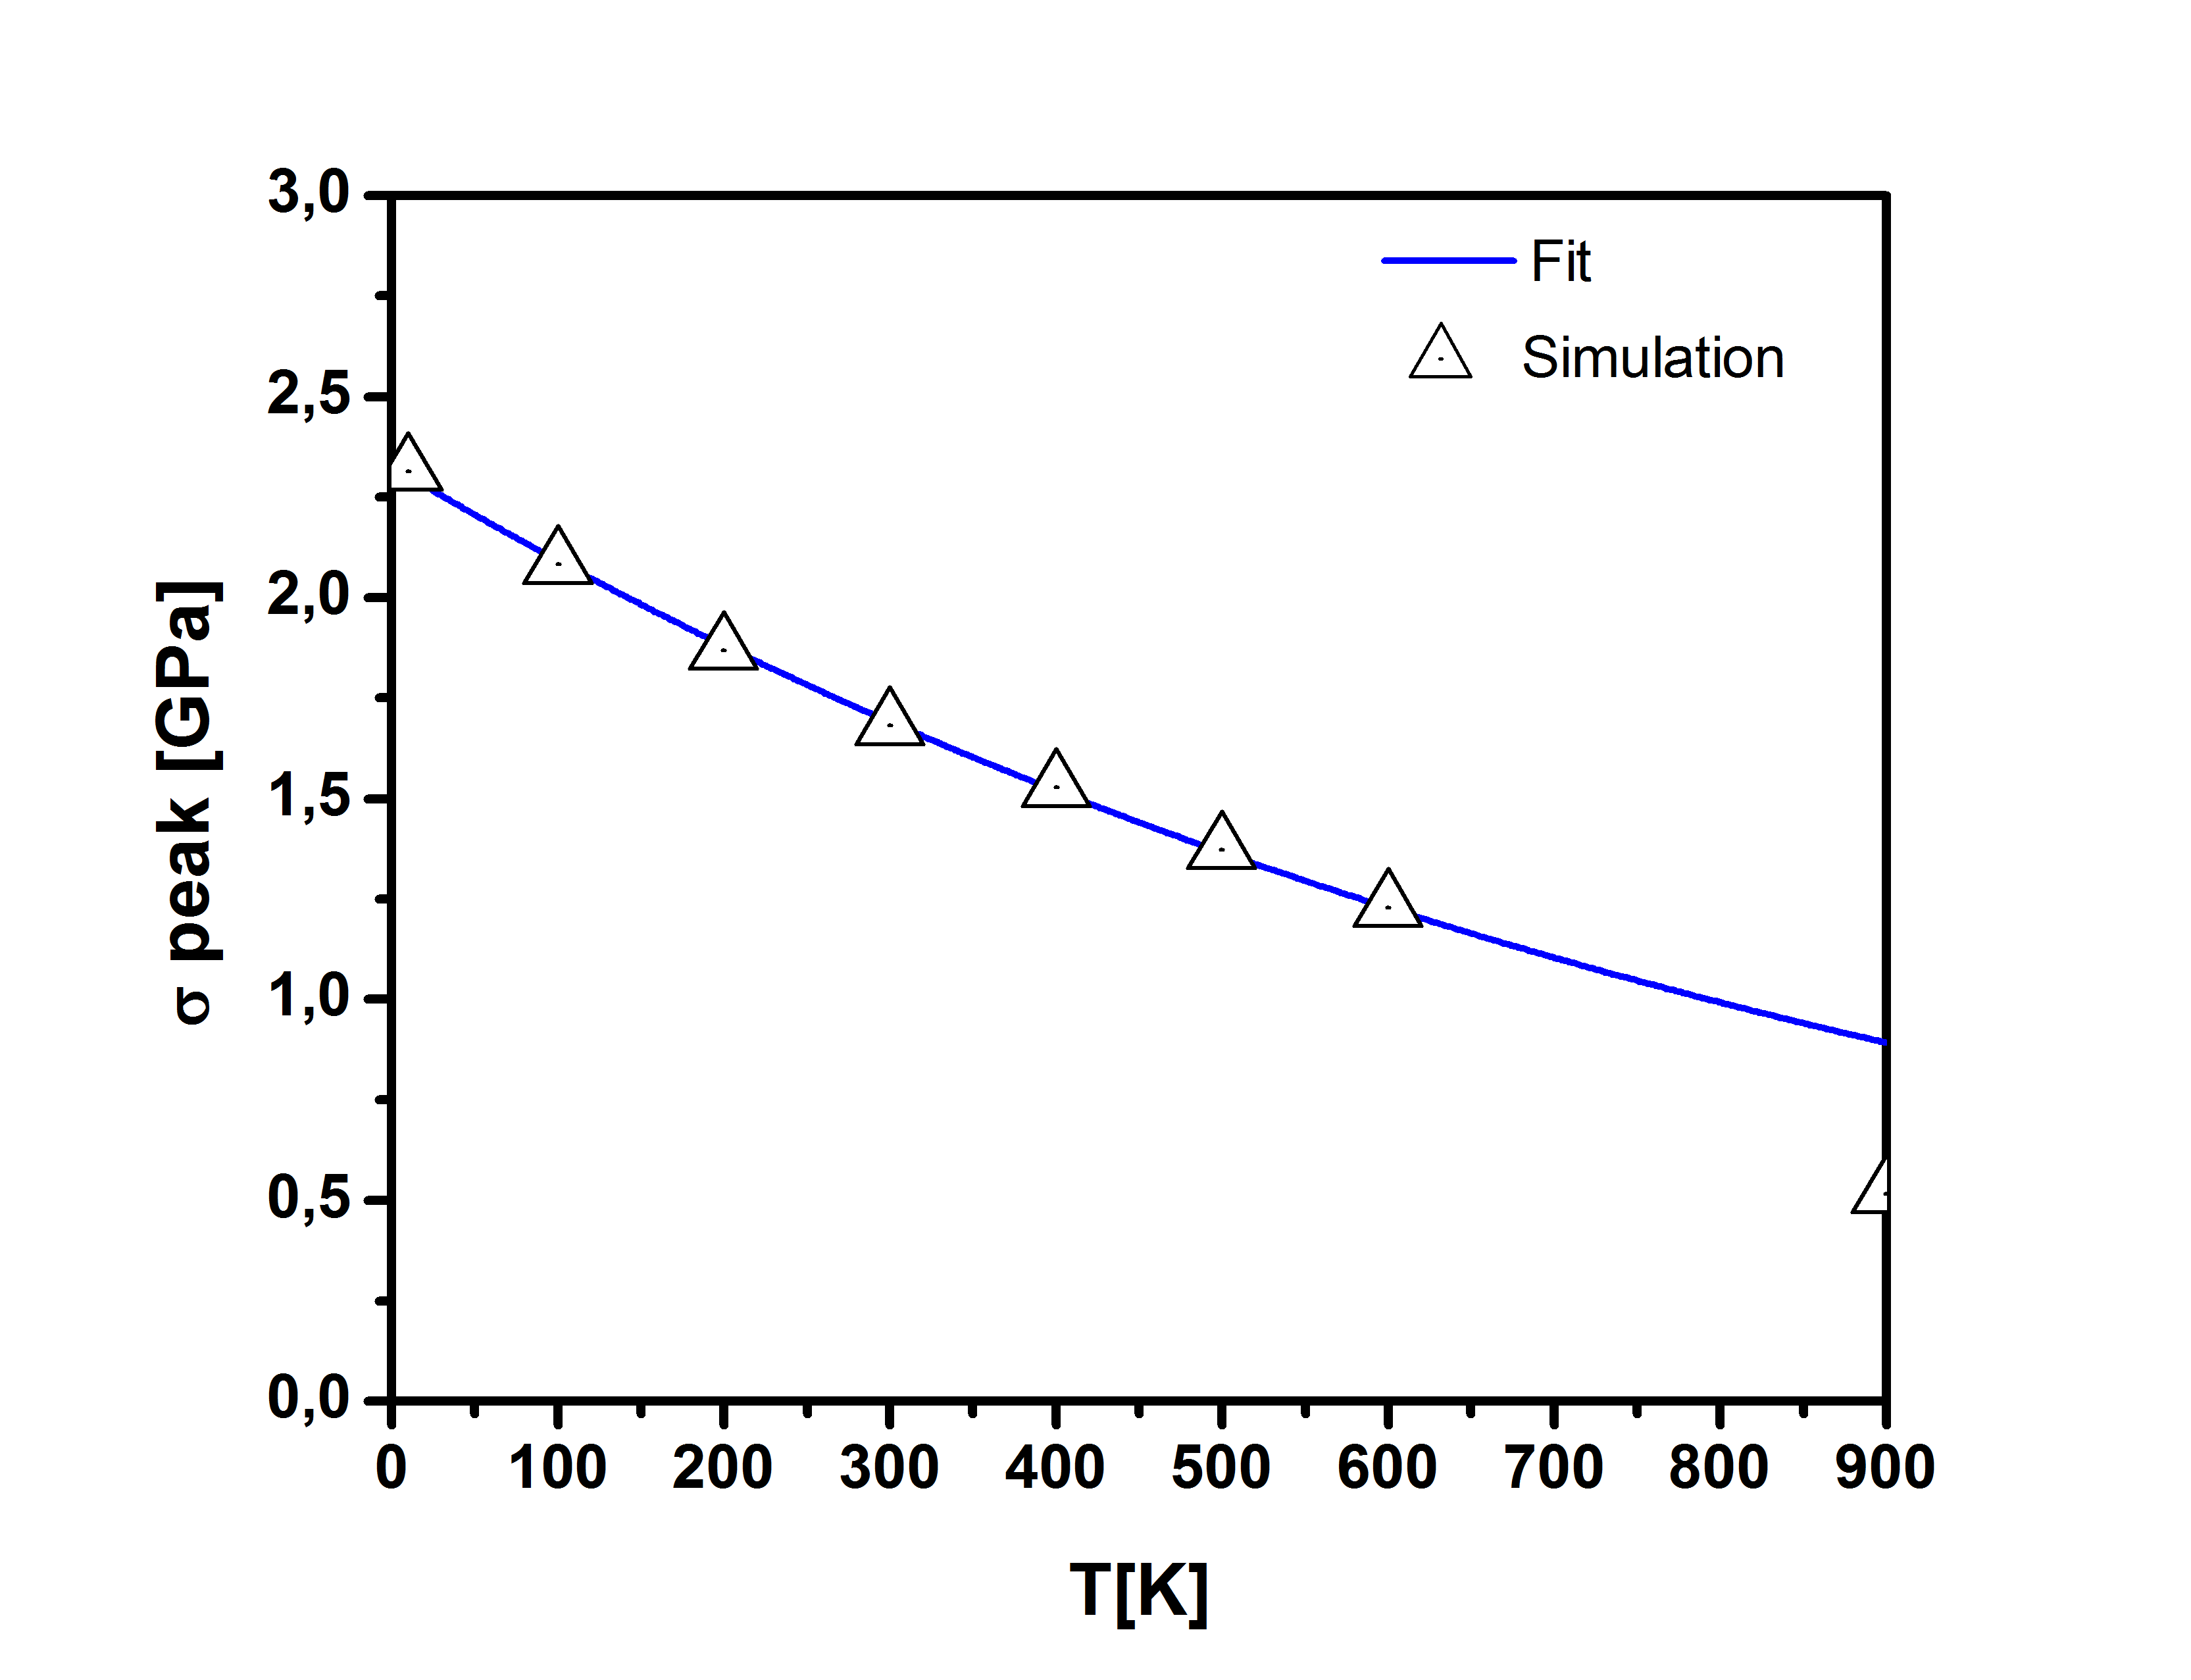
\includegraphics[width=8cm]{peakstress_T_TEN.png}
\caption{Von Mises maximo vs. Temperatura}
\end{figure}

\begin{figure}[H]
\centering
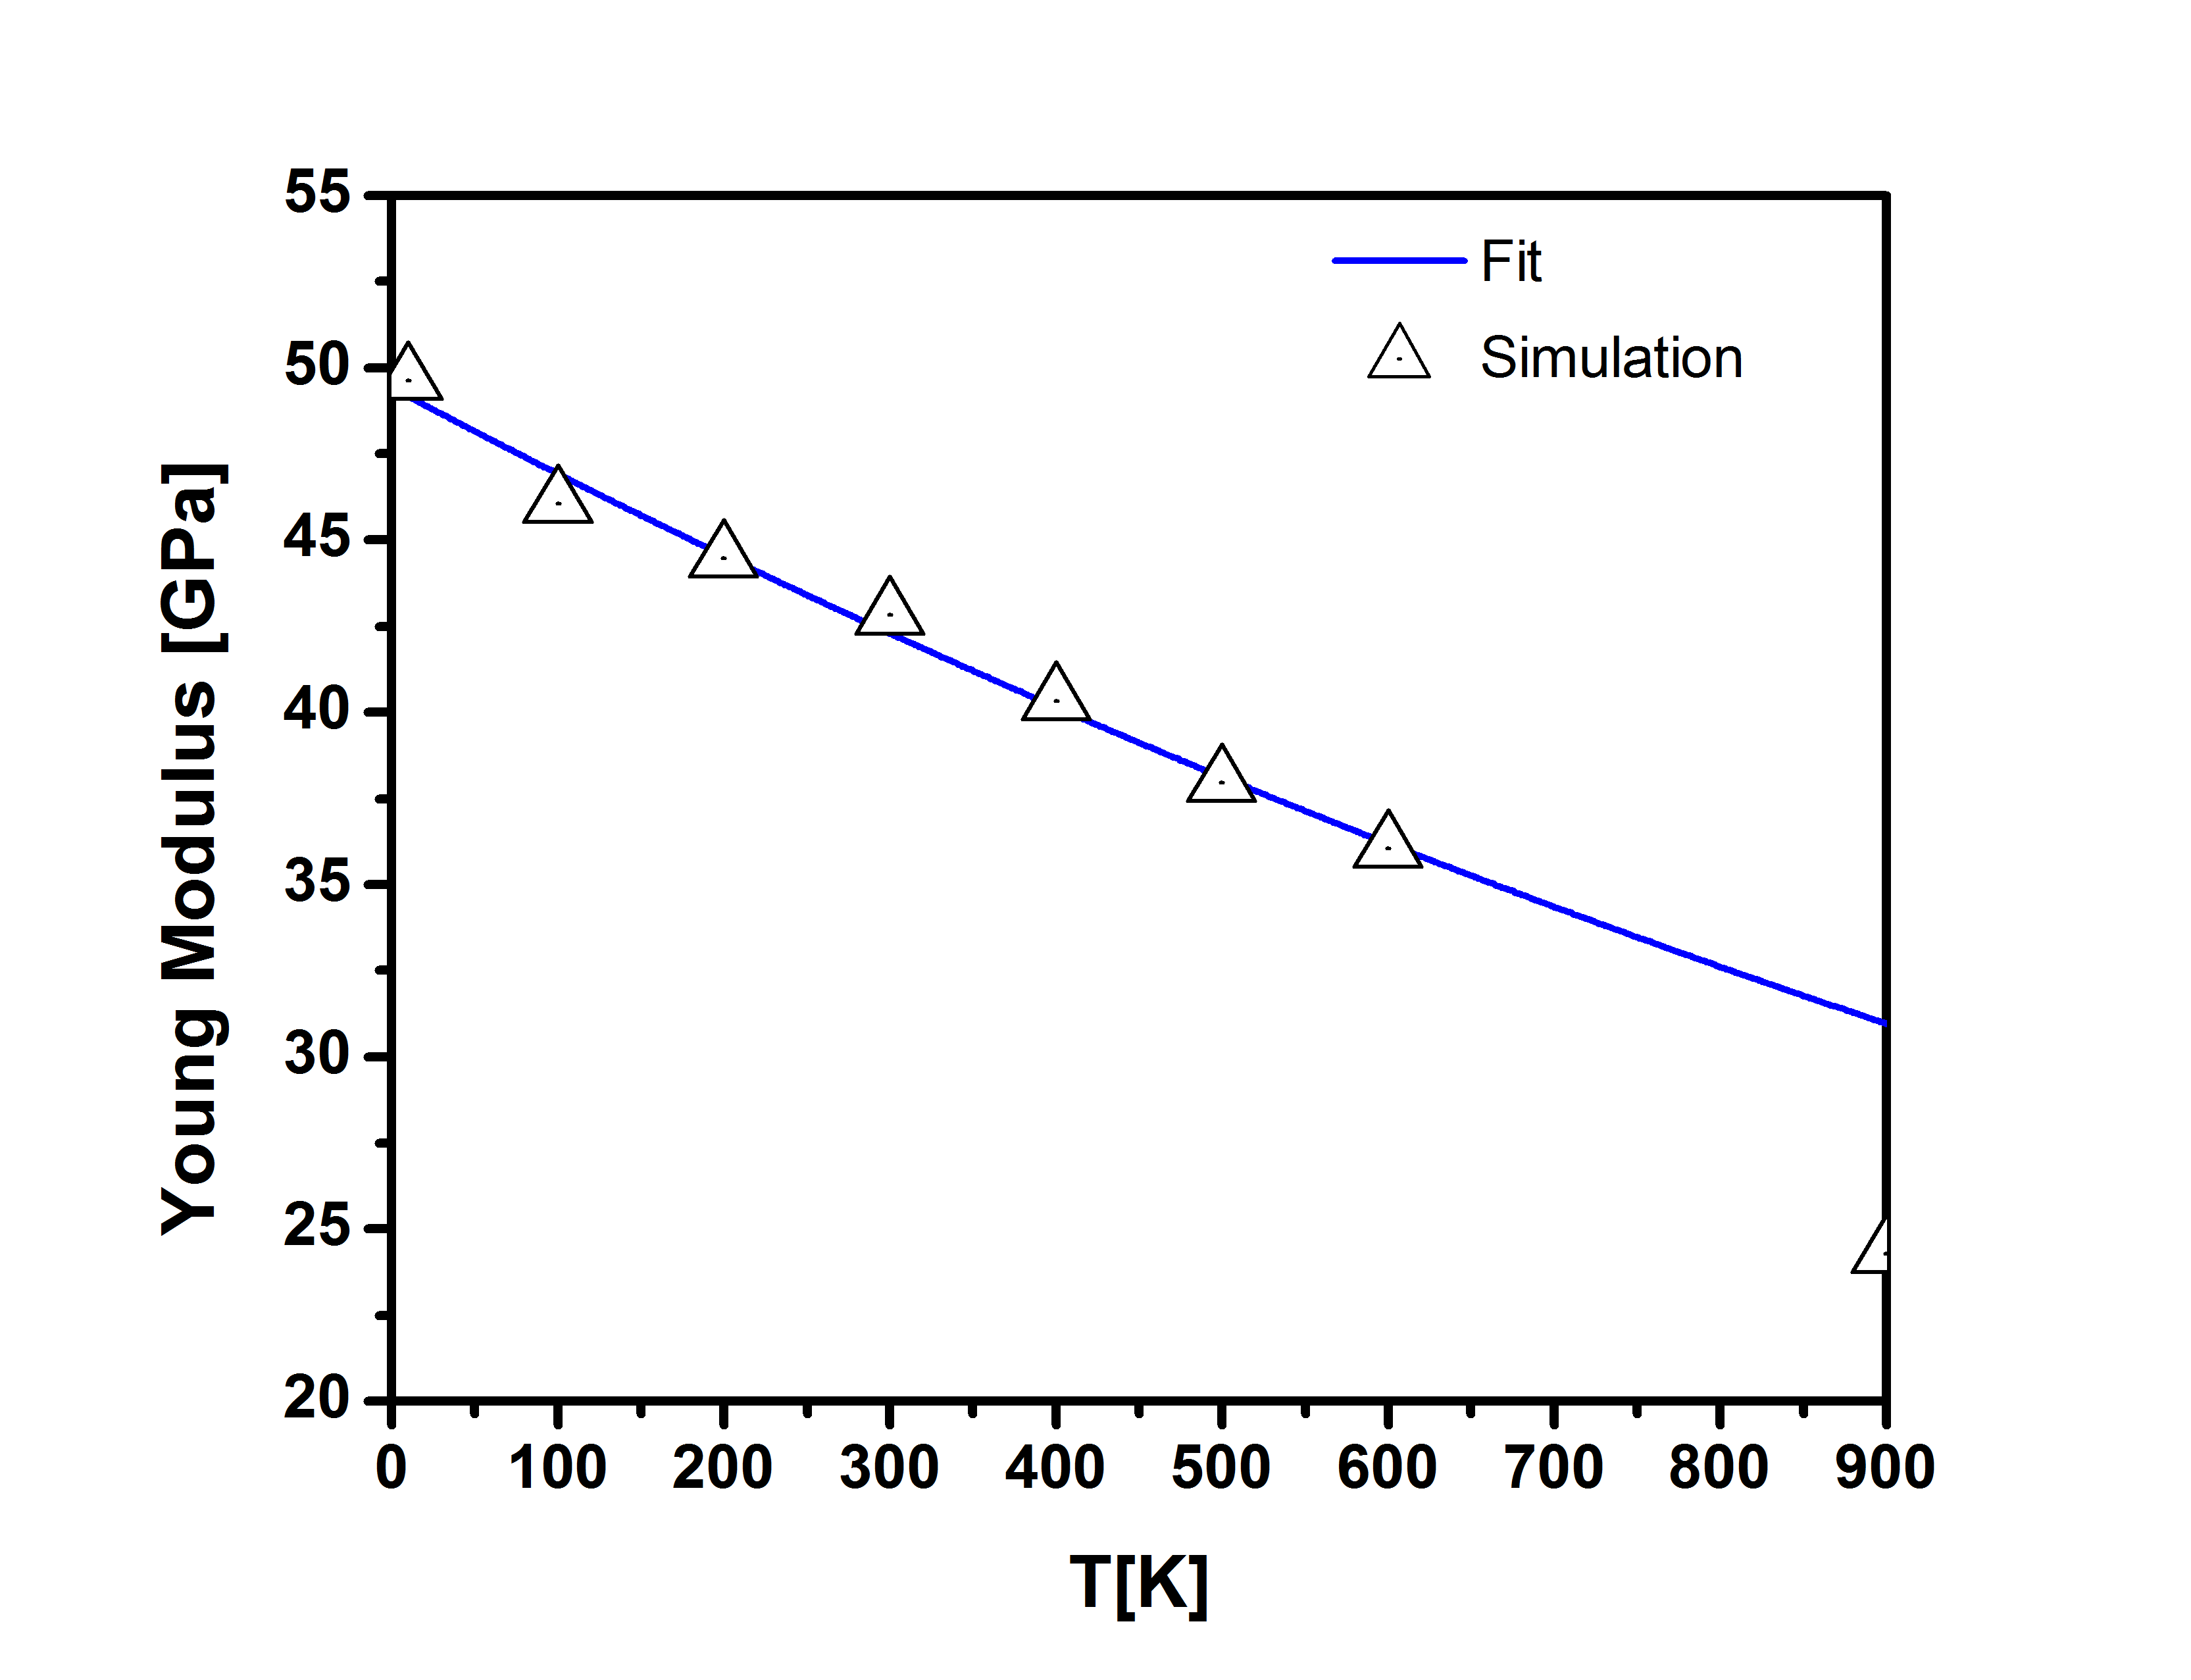
\includegraphics[width=8cm]{young_T_TEN.png}
\caption{Modulo Young vs. Temperatura}
\end{figure}

\end{document}
